% Created 2017-04-19 Wed 17:21
% Intended LaTeX compiler: xelatex
\documentclass[a4paper, notitlepage]{report}
\usepackage{graphicx}
\usepackage{grffile}
\usepackage{longtable}
\usepackage{wrapfig}
\usepackage{rotating}
\usepackage[normalem]{ulem}
\usepackage{amsmath}
\usepackage{textcomp}
\usepackage{amssymb}
\usepackage{capt-of}
\usepackage{hyperref}
% set the margins here, if they need to be modified
\usepackage[a4paper, left=1.3in, right=1.0in]{geometry}

% The linespacing you want
\linespread{1.4}

% Lets you pick fonts. Only works if you compile with xelatex or luatex
\usepackage[no-math]{fontspec}

% For block quotes
\usepackage{attrib}

% Additional mathsy symbols
\usepackage{amsmath}
\usepackage{amssymb}

% Used to make the captions on figures sans serif
\usepackage{caption}

% For including images
\usepackage{graphicx}

% For fancy code listings
\usepackage{listings}

% For tables that span multiple pages elegantly
\usepackage{longtable}

% For APA-style citations

% For maintaining a list of abbreviations
\usepackage{nomencl}

% For drawing diagrams
\usepackage{tikz}

% These closely match the SCSS word template fonts
% Won't work unless you compile with xelatex or luatex
\setmainfont[Mapping=tex-text]{Times New Roman}
\setsansfont{Helvetica}
\setmonofont{Courier New}

\pagestyle{headings}

\hypersetup{
    colorlinks,
    citecolor=black,
    filecolor=black,
    linkcolor=black,
    urlcolor=black
}

\bibliographystyle{acm}

% Settings for how you want your code listings to look
\lstset{
basicstyle=\ttfamily\scriptsize,
keywordstyle=\ttfamily,
numberstyle=\rmfamily\tiny,
numbers=left,
commentstyle=\sffamily,
breaklines=true,
frame=single,
stringstyle=\ttfamily,
identifierstyle=\bfseries,
lineskip=1mm
}

% Change these as appropriate, and they'll be filled in automatically on the
% cover page. You can also use them throughout the document, so as not to have
% to type them again all the time.
\newcommand \authorname{Brian McNestry}
\newcommand \authoremail{mcnestrb@tcd.ie}
\newcommand \supervisorname{Dr. Donal O'Mahony}
\newcommand \degreetitle{B.A. (Mod.) Integrated Computer Science}
\newcommand \projecttitle{Electricity Trading Between Smart Nano-Grids: \newline Matching Supply and Demand in the Face of Unpredictable Supply}

% All the commands are defined in this file
\newcommand \inserttitlepage{\thispagestyle{empty}
\begin{center}
{\sffamily
{\Large University of Dublin}

\vspace{10pt}


\includegraphics[scale=0.5]{tcd/trinitycollege.pdf}

\vspace{10pt}

{\Huge TRINITY COLLEGE}

\vspace{80pt}

\textbf{ \Large \emph \projecttitle}

\vspace{30pt}

\authorname

\degreetitle

Final Year Project May 2017

Supervisor: \supervisorname

\vspace{100pt}

\large{School of Computer Science and Statistics
\\$ $\\
O'Reilly Institute, Trinity College, Dublin 2, Ireland}
\linespread{1}
}
\end{center}

}
\newcommand \insertabstract{\begin{abstract}
\thispagestyle{plain}
As fossil fuels across the world are steadily depleted, the majority of the
world's energy production will shift towards renewable sources. However,
renewable energy sources do not always guarantee the same reliability in rates
of production. Therefore new strategies must be developed to match supply and
demand in the face of unpredictable supply. The growing popularity and
proliferation of smart grid technology is one proposed method of solving this
problem.

In this paper, a network implementation of a game theoretic approach to this
problem is implemented in a smart nanogrid to prove whether or not such an
approach is first feasible in a network, and secondly whether or not it would
provide a better approach to the problem. A number of optimisation techniques,
such as convex optimisation and hyperplane projection optimisation, are also
employed to find a better solution. 
\end{abstract}
}
\newcommand \declaration{\chapter*{Declaration}

I hereby declare that this project is entirely my own work and that it has not
been submitted as an exercise for a degree at this or any other university.
$ $\\
$ $\\
\signedanddate
}
\newcommand \acknowledgements{\chapter*{Acknowledgements}

Acknowledge the various people here
}
\newcommand \permissiontolend{\chapter*{Permission to lend}

I agree that the Library and other agents of the College may lend or copy
this report upon request.

$ $\\
$ $\\
\signedanddate
}

\newcommand{\argmax}[1]{\underset{#1}{\operatorname{arg}\,\operatorname{max}}\;}

\usepackage{datetime}

\def\fullhrulefill{\leavevmode\leaders\hrule height 1pt\hfill\kern 0pt}

\newcommand{\signedanddate} {
  \par\noindent\makebox[2.5in]{\fullhrulefill}
  \par\noindent\makebox[2.5in][l]{\authorname, May 5 2017}
}

\newcommand \needcite[1]{\underline{#1}}

\newcommand \abbrev[2]{#1\nomenclature{#1}{#2}}


% For changing the names of the List of Listings, etc.
\renewcommand*{\lstlistlistingname}{List of Listings}
\renewcommand*{\contentsname}{Table of Contents}
\renewcommand*{\nomname}{Abbreviations}

% Make the captions sans serif
\renewcommand{\captionfont}{\sffamily}

\addbibresource{bibliography.bib}
\author{Brian McNestry}
\date{\today}
\title{}
\hypersetup{
 pdfauthor={Brian McNestry},
 pdftitle={},
 pdfkeywords={},
 pdfsubject={},
 pdfcreator={Emacs 24.5.1 (Org mode 9.0.5)}, 
 pdflang={English}}
\begin{document}

\inserttitlepage

\pagenumbering{roman}

\declaration

\permissiontolend

\insertabstract

\acknowledgements

\tableofcontents

\newpage


\pagenumbering{arabic}

\part{Abstract}
\label{sec:org22dbc26}

\part{Introduction}
\label{sec:org5619b3d}


\part{Background}
\label{sec:org29888ff}
\chapter{Decentralised Grid}
\label{sec:orgf8a99f4}
At present in Ireland and in many other countries, the national electric grid
infrastructure is controlled by a central body, namely the ESB. While there are
several electricity providers in Ireland, such as Bord Gáis Energy, SSE
Airtricity and Energy Ireland, each of them use the same distribution network as
one another. Essentially the power is provided from each of the different
providers and then routed into the same centralised hub belonging to the ESB.
From there, each consumer (a household) receives the energy that they pay for
accordingly at a fixed rate through that same infrastructure belonging to the
ESB. This is much the same system as any other country, where there is a
centralised grid. 

This system has been in place for decades and lends itself very well to the
situation where large companies can provide a steady supply of energy by way of
electricity plants that use both renewable and non-renewable energy sources.
Non-renewable energy sources, also known as fossil fuels, include resources such
as coal, gas and oil. While these are finite resources, at present they can be
burned at a steady rate in order to meet the demands of customers. Electricity
from renewable sources can also be produced at a fairly steady rate by placing
large farms in areas that are particularly well suited to the type of renewable
energy being produced. For example, large wind farms are set up in windy
regions far removed from residential or urban areas and solar panels can be
placed in regions that typically enjoy clearer skies than other areas.

However in the future, perhaps the very near future, with the ongoing depletion
of non-renewable resources, more and more people will turn to deploying solar
panels and local wind farms in their locale, regardless of whether or not they
are living in a particularly sunny or windy area. At the moment there are a few
houses out there that use a solar panel to heat their water or other smaller
tasks but soon more and more people will become more and more dependent on what
they can produce either within their own home, or in a more collective sense in
their own neighbourhood to power their houses.

The issue that then arises in these areas that aren't as sunny or windy is that
supply of electricity is no longer steady. The current system could not be
maintained as the energy produced on a local level would be small enough that it
would not be worth it to pass this energy upstream to the central grid. The
energy would instead be used at a local level to try to cover the demand for
electricity of the house or business with which that particular device is
associated.

The model of infrastructure that would then be required is that of a
decentralised grid. This model would need a massive infrastructure overhaul in
order to implement so it would not exist in the world until it is needed and
accepted by the major companies who would then go about implementing it. In this
case necessity would be the mother of invention, at least on a practical level.
The rough idea of a distributed grid is described in figure 1.1. Throughout the
rest of this report distributed grid and decentralised grid are used
interchangeably. 

\begin{figure}[htbp]
\centering
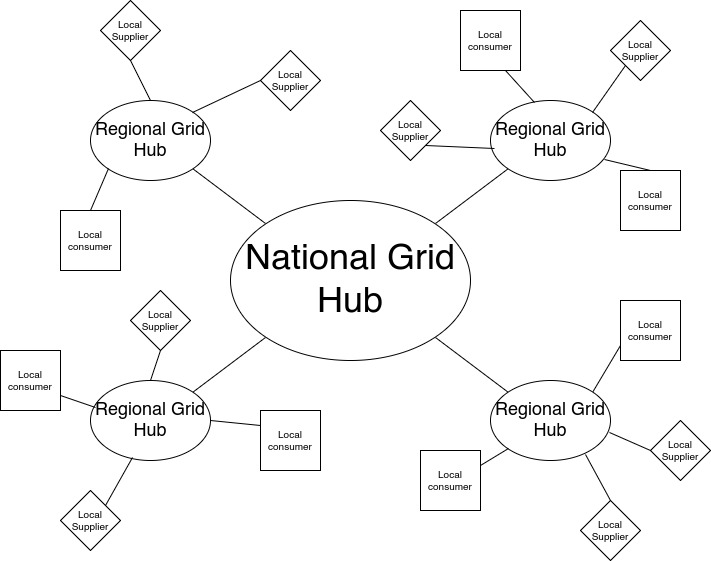
\includegraphics[width=.9\linewidth]{./img/DecentralisedGrid.jpg}
\caption{\label{fig:org7c128db}
Each local consumer and supplier is attached to a regional grid hub which manages the allocation of electricity between suppliers and consumers. This is just a simple overview of the idea but conceivably a consumer or a supplier could be connected to two or more different regional grid hubs.}
\end{figure}
\chapter{Smart Grid}
\label{sec:orgc17f186}
\section{Overview}
\label{sec:org1423fb1}
Due to advancements in networking technologies as well as in the field of
sophisticated decision making technologies, the idea of a smart grid has become
increasingly popular. The idea of the smart grid is that actors within a grid,
be they individual consumers or suppliers, or groups thereof, can be fitted with
small computers that perceive changes in the grid and then these actors can
then react accordingly. Several different types of management systems have been
constructed in order to successfully, fairly and efficiently allocate resources
for each of these different types of actors. The two primary types of management
systems that were examined as part of this final year project were Auctions and
Game Theory which will both be discussed in detail later on.

The smart grid is not only used in this regard but in fact has many other
potential applications, some of which have been implemented already in several
cities and regions throughout the world. Other applications of the technology
include energy consumption or production prediction, scheduling the use of
consumers in order to reduce costs or operation and smart reaction and response
to disruptions or blackout within the grid to reduce the damage that occurs as a
result.

In this project it is assumed that the consumers within the system are outfitted
with some kind of prediction technology. An example of such a system has been
proposed by Garcia et al \cite{mohsenian2010optimal} where a device tries to time
its own operation within a certain time-frame in accordance with when the price
of energy is cheapest. It also tries to predict how much energy it will consume
based off its own knowledge of previous experiences in buying power at that
particular time of day, allowing the system to learn over time and make smarter
decisions as time goes on.

\section{Microgrids and Nanogrids}
\label{sec:org77c43aa}
At present smart grids have generally been implemented on the level of
microgrids. Microgrids are generally thought of in terms of having a consumer
be a single house, or perhaps a group of houses, and a supplier being a small
wind farm or solar farm, or perhaps a group of these together. In the case of a
microgrid, actors within the system are defined in similar to the units involved
in a centralised grid system meaning that the transition from a centralised grid
to the microgrid scheme was a relatively easy one.

An example of such a real world implementation is that of the system in place in
Japan. This system was mostly implemented following the disaster of Fukushima,
where it became clear that a reliance on a single power source and a centralised
power distribution network left the country vulnerable following the disaster
\cite{japan_microgrids}. Several regions were cut off from power as a result of
the disaster which hampered the relief efforts as well as making the lives of
ordinary Japanese citizens more difficult. Had a microgrid system been in place
then not so many hospitals and homes would have been left without power
following the disaster. The company ENEL has also introduced a smart grid system
in the region of Apulia in southern Italy \cite{sapienza2013enel}.  

The nanogrid system is very similar to that of the microgrid system conceptually
but is concerned with a much smaller scale. A nanogrid is one that operates
within the confines of a single building, generally where each consumer is a
single appliance such as a washing machine or an electronic vehicles (EV).
Suppliers would also be very small scale perhaps a set of solar panels or a
small wind turbine. A nanogrid system could also be adapted to aggregate a number
of devices to act as one as a single actor within the nanogrid system, for
example all the lights on one floor of a house could act as a single consumer
and draw on a shared reserve of power.

Another extension of the nanogrid system, which will be discussed in further
detail in the conclusion section of this paper, would be to incorporate a
nanogrid as a sub-node of a microgrid. This would create a hierarchy of
distributed grids. This tree could also be adapted into a graph where a parent
node in the tree could have multiple children and a child could have multiple
parents. This will be discussed more in the conclusion.
\chapter{REFIT Scheme}
\label{sec:org1181de5}
\chapter{Auctions}
\label{sec:orgc17a68d}
\chapter{Game Theory}
\label{sec:orgfc6e072}
\section{Overview}
\label{sec:orga508f04}
The field of game theory has been one that has many different facets and
versions depending on the type of situation required. In this section of the
report the nomenclature and jargon of game theory will be discussed, as will a
short explanation about the decision of selection of the type of game
implemented as part of this final year project. First the two primary types of
interactions between players in a game will be discussed and after that the two
primary types of playing styles will be discussed. However first of all there
are certain traits that are universal for any type of game that must first be
explained in order to grasp the concept of game theory enough to understand some
of the implementation decisions later in this report as well as to grasp the
general concept of game theory itself.

In game theory, players within a game compete for a finite resource with the
objective of maximising their own utility within the scope of that game. Each
player within the game has an associated utility function that is generally the
same for all players within that game. The utility function generally results in
some scalar value that is trying to reach some max value, whether on an
individual or collective level. There is also generally some kind of manager
node that helps to conduct the game between all of the players involved. Within
any particular game, the players are all trying to maximise their own utility,
however in different types of games they may also be conscious of the utilities
of all the other players involved and try to react accordingly, whether to
further their own goal or to further the goals of the collective group.

A well defined game also has some from of state of equilibrium. This state of
equilibrium is when the sum of utilities of all the players within the game
reaches a maximum. The central managing node, if there is one, generally decides
whether or not this state has been reached. This state is the success state of
the game. In a well-designed game the utility function must be designed such
that the state of equilibrium not only can be reached but also that reaching
that state is appealing to all players within the game.
\section{Non-Cooperative Game Theory}
\label{sec:org4d72ccd}
Non-Cooperative games are the simplest types of games to both understand and
design. As previously stated, each player is trying to maximise its own utility
but the core component of a non-cooperative game is that all of the players are
operating purely independently. Each player within the game knows the best
strategy to take in order to maximise its own utility. Because each player in a
game has the same moves open for them to take and therefore the same strategy
that each other player will take to maximise their own respective utilities.

This is where the concept of Nash Equilibrium comes into play. Nash Equilibrium
is the state in which there is the least disparity between the best player and
the worst player, that is that each player performs the best that it can with
the knowledge that all other players are similarly going to try to maximise
their own utilities. With this knowledge, each player is then able to pick the
strategy that maximises its own utility, taking into consideration that all
other players are trying to do the exact same thing and therefore it picks an
appropriate strategy. In a well designed game, there should also be no incentive
for a player to change their strategy to try to undercut other players. If made
correctly, such an action would have an adverse effect on the player in the
game. In this case all other players would then be aware that this players
strategy had changed and would then react accordingly in order to maximise their
own utility and decrease that player's utility.
\section{Cooperative Game Theory}
\label{sec:org9e3de17}
Cooperative game theory shares many similar traits with that of non-cooperative
game theory as outlined in the overview section of this part on game theory in
this report. However the key aspect of cooperative game theory is that players
within the game will form coalitions based on threats and incentives that occur
between each other. The key component of cooperative game theory is the
analysis of which coalitions are likely to form within any given game and what
the projected outcomes are based upon these permutations of coalitions. In this
way the study of cooperative games have two main facets. First of all they are
concerned with what might cause different groups of players to act together in
unison. Secondly they are concerned with the outcomes from the most likely of
each of these games that happen when different groups form.

In this project, the nodes involved in the game are all energy suppliers who are
each trying to maximise their own profit based on the amount of energy that they
are able to sell. The utility functions of the nodes and other such details will
be discussed later in the Implementation section of this report. The desired
outcome of each player is therefore entirely selfish and because they are all
trying to compete for a finite price, they each want to obtain as much of that
money as possible. Therefore it does not make sense to design this game in such
a way that these players should be able to form coalitions, as any coalition
would involve compromising and receiving less money which doesn't make sense in
this game. Similarly due to the lack of communication between the players in the
game, they can also never know if other players could change their strategies so
are unable to even realise that cooperation is even possible at any given stage.
\section{Cournot and Stackelberg Games}
\label{sec:org72c12c9}
\chapter{Optimisation Techniques}
\label{sec:org6177a74}
\section{Convex Optimisation}
\label{sec:orga46ecbf}
\section{Hyperplane Projection}
\label{sec:orgff4fd09}
\part{Implementation}
\label{sec:orga51a39c}
\chapter{Design}
\label{sec:org1ae0535}
\chapter{Framework}
\label{sec:org6bb7567}
\chapter{Processes}
\label{sec:orgde468b3}
\part{Conclusion}
\label{sec:orgcd39caf}
\chapter{Assessment}
\label{sec:org1d5837b}
\chapter{Future Work and Continuations}
\label{sec:orgb6bec35}
\printbibliography
\appendix
\end{document}